\documentclass[a4paper,12pt]{report}
\usepackage[hidelinks]{hyperref}
\usepackage{float}
\usepackage{graphicx}
\usepackage{listings}
\usepackage[utf8]{inputenc}
\usepackage{etoolbox}
\usepackage{fullpage}
\renewcommand*\contentsname{Indice}
\usepackage{setspace}
\usepackage{parskip}
\usepackage{amsmath}

% un po' di estetica...
\usepackage{fancyhdr}
\pagestyle{fancy}
\setlength{\headsep}{0.35in}
\let\MakeUppercase\relax

% blocchi di codice
\usepackage{listings}
\lstset{
	breaklines=true, 
	frame=single, 
	numbers=left,
	tabsize=2,
	basicstyle=\scriptsize,
	showstringspaces=false
}

\setlength{\parindent}{2em}
\setlength{\parskip}{0.5em}
\renewcommand{\baselinestretch}{1.5}

\fancyhf{} % clear all fields
\fancyfoot[C]{\thepage}

\frenchspacing

\newcommand{\mychapter}[2]{
    \setcounter{chapter}{#1}
    \setcounter{section}{0}
    \chapter*{#2}
    \addcontentsline{toc}{chapter}{#2}
}

\begin{document}

\begin{titlepage}
\noindent
    \vspace*{5mm}
	\begin{minipage}[t]{0.15\textwidth}
	    \vspace*{5mm}
		\vspace{-3.5mm}{
\includegraphics[scale=1.8]{../img/logo_bicocca.png}}
	\end{minipage}
	\hspace{1cm}
	\begin{minipage}[t]{0.9\textwidth}
	      \vspace*{5mm}
		{
			\setstretch{1.42}
			{\textsc{Università degli Studi di Milano - Bicocca} } \\
			\textbf{Scuola di Scienze} \\
			\textbf{Dipartimento di Informatica, Sistemistica e Comunicazione} \\
			\textbf{Corso di Laurea Magistrale in Informatica} \\
			\par
		}
	\end{minipage}
	
	\vspace{42mm}

\begin{center}
    {\LARGE{
	    	\setstretch{2}
            \textbf{
            	Metodi del Calcolo Scientifico - Progetto 2 \\ 
            	Compressione di immagini tramite la DCT \\ }
    }}        
\end{center}

\vspace{40mm}
	
	
	\begin{flushright}
		\setstretch{1.3}
		\large{Alberici Federico - 808058\\} 
		\large{Bettini Ivo Junior - 806878\\} 
		\large{Cocca Umberto - 807191\\} 
		\large{Traversa Silvia - 816435} 
	\end{flushright}
	
	\vspace{15mm}
	\begin{center}
		{\large{\bf Anno Accademico 2019 - 2020}}
	\end{center}


\renewcommand{\baselinestretch}{1.5}

\end{titlepage}

\tableofcontents

\mychapter{0}{Introduzione}
In questa relazione vengono presentate e discusse le modalita di implementazione della DCT (dall'inglese Discrete Cosine Transform), ovvero la più diffusa funzione che provvede alla compressione spaziale.\\
Nella prima parte viene confrontata la versione "Nativa" della DCT con alcune varianti conosciute, studiandone il costo computazionale.\\
Nella seconda parte viene documentato un semplice tool per applicare su immagini in toni di grigio, tramite un approccio di compressione tipo jpeg (senza utilizzare una matrice di quantizzazione), la funzione DCT2 implemetata.

\mychapter{1}{Analisi DCT}

\section{Discrete Cosine Transform}
Una DCT esprime una sequenza finita di punti in termini di una somma di funzioni coseno oscillanti a diverse frequenze. Ad oggi è una delle tecniche di trasformazione piu utlizzate nella Teoria dei segnali e nella compressione dei dati, in particolare nei media digitali (audio, video, radio ecc..).\\
In queste applicazioni infatti la maggior parte delle informazioni significative tendono ad essere concentrate in poche componenti a bassa frequenza della DCT. Questo permette di comprimere a piacere il dato scartando le componenti ad alta frequenza (compressione lossy).

\section{DCT-II e DCT-III}
La DCT-II è probabilmente la forma più utilizzata, infatti viene indicata come "la DCT".\\
\[X_k = \sum_{n=0}^{N-1} x_n \cos \left[\frac{\pi}{N} \left(n+\frac{1}{2}\right) k \right] \quad \quad k = 0, \dots, N-1.\]\\\\
La sua inversa è la DCT-III e per questo viene indicata come "l'inversa della DCT" o "IDCT".\\
\[X_k = \frac{1}{2} x_0 + \sum_{n=1}^{N-1} x_n \cos \left[\frac{\pi}{N} n \left(k+\frac{1}{2}\right) \right] \quad \quad k = 0, \dots, N-1.\]\\\\
Entrambe le funzioni effettuano N somme per calcolare la k-esima componente di un vettore di N componenti, determinando un costo computazionale \( O(N^2)\).

\subsection*{Implementazione}

\section{DCT tipo I - IV}

\section{DCT di Lee}

\section{Confronto}
%Creazione codice e descrizione libreria
%commento confronto
\begin{figure}[H]
\centering
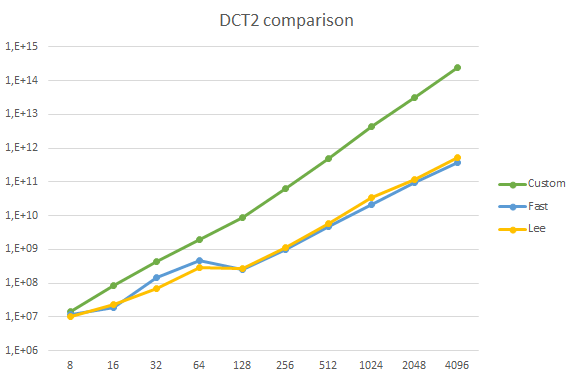
\includegraphics[width=0.77\linewidth]{../img/comparison.png}
%\caption{\textit{}}
\label{fig:2}
\end{figure}

\mychapter{2}{Test con immagini}

\section{Tool di testing}

\section{Risultati}
\end{document}